%! TEX root = ../../master.tex

\lecture[Satz von Seifert van Kampen. Wiederholung: Pushouts. Freie und amalgisierte Produkte von Gruppen als Pushouts in $\Grp$. Die Fundamentalgruppe  $F_2$ von  $S^1 \twedge S^1$. Konstruktion von Räumen mit 'fast' freier Fundamentalgruppe.]{Do 01 Jul 2021}[20]{Seifert van Kampen}[Fortsetzung]

\section{Der Satz von Seifert von Kampen}\label{sec:seifert-van-kampen}

\begin{restatable}[Seifert-van-Kampen]{theorem}{ThmSeifertVanKampen}\label{thm:seifert-van-kampen}
    Sei $X$ ein Raum, seien  $U_1,U_2\subset X$ offen, sodass $U_1\cup U_2 = X$, und bezeichne  $U_3 \coloneqq  U_1 \cap U_2$.

    Sind $U_1,U_2,U_3$ wegzusammenhängend und nicht-leer sowie $x_0\in U_3$, dann ist
    \[
        \begin{tikzcd}[ampersand replacement = \&]
        \pi_1(U_3,x_0) \ar[swap]{d}{} \ar{r}{} \& \pi_1(U_1,x_0) \ar{d}{} \\
        \pi_1(U_2,x_0) \ar[swap]{r}{} \& \pi_1(X,x_0)
    \end{tikzcd}
    l\]
    ein Pushout von Gruppen, d.h. für jede Gruppe $H$ und kompatible Morphismen  $\pi_1(U_1,x_0) \to  H$ sowie $\pi_1(U_2,x_0) \to  H$ existiert ein eindeutig bestimmter Morphismus $\pi_1(X,x_0) \to  H$. Visualisiert:
    \[
        \begin{tikzcd}[ampersand replacement = \&]
        \pi_1(U_3,x_0) \ar[swap]{d}{} \ar{r}{} \& \pi_1(U_1,x_0) \ar{d}{} \\
        \pi_1(U_2,x_0) \ar[swap]{r}{} \& \pi_1(X,x_0)
    \end{tikzcd}
    \]
\end{restatable}



Wir geben zunächst einige Erklärungen und Beispiele zu \autoref{thm:seifert-van-kampen}:

\begin{remark}
    Ein Pushout in Gruppen ist ein sogenanntes \textit{amalgisiertes Produkt}, d.h.
    \[
    \begin{tikzcd}
        H \ar[swap]{d}{} \ar{r}{} & G_1 \ar{d}{} \\
        G_2 \ar[swap]{r}{} & G_1 \star_H G_2
    \end{tikzcd}
    \]
    ist ein Pushout.
\end{remark}

\begin{ddefinition}[Amalgisiertes Produkt]
    Seien $G_1,G_2$ zwei Gruppen. Sind $G_i = \left< E_i \mid  R_i \right> $ Darstellungen der Gruppen, so ist das \vocab{freie Produkt} von $G_1$ und $G_2$ die Gruppe bestimmt durch
    \[
G_1 \star G_2 \coloneqq      \left< E_1 \cup E_2\mid R_1 \cup R_2 \right> 
    .\] 
    ,d.h. die Menge aller (endlichen) Wörter mit Elementen aus $G_1$ und $G_2$ mit den kanonischen Verknupfungen von Elementen aus $G_1,G_2$, aber keinerlei weiteren Relationen.

    Sind $\varphi_1\colon H \to  G_1$ und $\varphi_2\colon H\to G_2$ Gruppenhomomorphismen, so ist das \vocab{amalgasierte Produkt} von $G_1$ und $G_2$ über $H$ (mit den Morphismen  $\varphi_1,\varphi_2$) definiert als
\[
    G_1\star_H G_2 \coloneqq  \faktor{G_1 \star G_2}{\varphi_1(h) \sim  \varphi_2(h)}
.\] 
\end{ddefinition}

\begin{example}\label{ex:fundamentalgruppe-von-s1-wedge-s1}
    Betrachte $S^1 \twedge S^1$, wir wollen $\pi_1(S^1 \twedge S^1, 1)$ berechnen, und haben dazu $U_1 = ι_1(S^1)$ und $U_2 = ι_2(S^1)$, dann sind beide offenen Mengen nichtleer und wegzusammenhängend, und es ist $U_1 \cap U_2 = \left \{1\right\} $ einelementig. Also ergibt sich
    \[
        \pi_1(S^1 \twedge S^1,1) \cong \pi_1(S^1,1) \star_{\pi_1(\left \{1\right\} ,1)} \pi_1(S^1,1) \cong \pi_1(S^1,1) \star \pi_1(S^1,1) \cong \mathbb{Z} \star \mathbb{Z} \cong F_2 = \left< a,b \right> 
    .\] 
    \begin{oral}
        Eigentlich hätten wir $U_1,U_2$ hier offen wählen müssen, um den Satz anwenden zu können. Die Umgebung 'ein bisschen' größer zu machen zerstört aber offensichtlich nichts an der Fundamentalgruppe von $S^1$, deswegen ist das in Ordnung und einfach ein formales Ausformulieren.
    \end{oral}
\end{example}

\begin{example}[Nicht-Beispiel]
    Der Wegzusammenhang ist essentiell!. Wenn wir $S^1 = D^1 \cup_{S^0} D^1$ schreiben, so ist der Schnitt nicht zusammenhängend, weswegen wir nicht die falsche Aussage
    \[
        \mathbb{Z} \cong \pi_1(S^1,1) \cong \pi_1(D^1,1) \star_{\pi_1(S^0,1)} \pi_1(D^1,1) \cong \left \{1\right\}  \star_{\left \{1\right\} \star \left \{1\right\} } \cong \left \{1\right\} 
    .\] 
    folgern.

    Es ist ebenfalls essentiell, die Offenheit zu fordern, sonst können wir z.B. $S^1$ einfach 'auftrennen'.
\end{example}


\begin{oral}
    Man kann die Aussage verallgemeinern und die Annahme des Wegzusammenhangs fallen lassen, wenn man statt den Fundamentalgruppen die Fundamentalgruppoide verwendet. Das ist aber nicht unser Ziel, weil dann die Pushouts deutich komplizierter werden.
\end{oral}

\begin{example}
    Sei $G = \left< a_1,\ldots,a_n\mid r \right> $ eine Gruppe auf $n$ Erzeugern und einer Relation  $r$. Wir wollen einen Raum konstruieren, der  $\pi_1(X,x_0) = G$ ergibt.

    Betrachte dazu
    \[
    Y \coloneqq  \bigvee_{i=1}^{n} S^1
    .\] 
    d.h. ein Zusammenkleben von $n$ Schleifen, dann erhalten wir $\pi_1(Y,1) \cong \left< a_1,\ldots,a_n \right> $ als freie Gruppe in $n$ Erzeugern (folgt induktiv aus \autoref{ex:fundamentalgruppe-von-s1-wedge-s1}). Wähle nun eine Schleife $S^1 \stackrel{f}{\longrightarrow} Y$, die $r$ repräsentiert. Definiere nun den Raum  $X$ als das Pushout
     \[
    \begin{tikzcd}
        S^1 \ar[swap]{d}{} \ar{r}{f} & Y \ar{d}{} \\
        D^2 \ar[swap]{r}{} & X
    \end{tikzcd}
    \]
   und betrachte
   \[
       U_1 \coloneqq  {D^2}\degree, \qquad U_2\coloneqq X \setminus \left \{\text{Mittelpunkt von $D^2$}\right\} \simeq Y
   .\] 
   Dann ist $U_3 \cong {D^2}\degree \setminus \left \{\text{Mittelpunkt}\right\} \simeq S^1$ und somit
   \[
       \pi_1(X) \cong \pi_1(U_1) \star_{\pi_1(U_3)} \pi_1(U_2) \cong \left \{1\right\} \star_{\mathbb{Z}} \pi_1(Y) \cong \faktor{\pi_1(Y)}{\left< \left< r \right>  \right> } = \left< a_1,\ldots,a_n|r \right>  = G
   .\] 
\end{example}

\lecture[Beispiele zu Seifert van Kampen.]{Di 06 Jul 2021}[21]{CW-Komplexe}

\begin{figure}[ht]
    \centering
    \incfig{skizze-zu-seifert-van-kampen}
    \caption{Skizze zu Seifert van Kampen}
    \label{fig:skizze-zu-seifert-van-kampen}
\end{figure}

Betrachte nun \autoref{fig:skizze-zu-seifert-van-kampen}, da 'sieht man' viel zur Intuition von Seifert van Kampen: Einen Weg $α$, der in  $X = U_1 \cup U_2$ verläuft, können wir aufteilen in einzelne kleinere Wege, die in $U_1$ oder $U_2$ verlaufen. Mit Hilfswegen $r_1,r_2$ machen wir daraus Schleifen an $x_0$, die nun in $U_1$ oder $U_2$ verlaufen. So erhalten wir bereits zumindest eine Projektion vom freien Produkt $\pi_1(U_1,x_0) \amalgprod  \pi_1(U_2, x_0)$ nach $\pi_1(X,x_0)$.

Wir erinnerns uns hier auch noch an \autoref{def:wedge-produkt}, das letztendlich auch nur ein Pushout von Räumen ist. Wir können also Seifert van Kampen auch umformulieren zu 'Seifert van Kampen erhält \textit{schöne} Pushouts'.

Wir können diese Intuition nun in einer kombinatorischer Form ausdrücken, hierzu sei $x_0\in U_3 \coloneqq  U_2 \cap U_1$ mit $U_1 \cup U_2 = X $ gegeben. Mit $\pi_1$ erhalten wir bereits ein Diagramm
\[
\begin{tikzcd}
    \pi_1(U_3, x_0)\ar[swap]{d}{\varphi_2 } \ar{r}{\varphi_1} & \pi_1(U_1,x_0) \\
    \pi_1(U_2,x_0)
\end{tikzcd}
\]

Wählen wir nun Gruppendarstellungen

\begin{IEEEeqnarray*}{rCl}
    \pi_1(U_1,x_0) & \cong & \left< α_1, \ldots, α_k \mid  r_1, \ldots, r_l \right> \\
    \pi_1(U_2,x_0) & \cong & \left< β_1, \ldots, β_m \mid  s_1, \ldots, s_n\right>  \\
    \pi_1(U_3,x_0) & \cong & \left< γ_1, \ldots, γ_p \mid  t_1, .., t_q \right> 
\end{IEEEeqnarray*}



\begin{corollary}\label{cor:seifert-van-kampen-für-einfach-zusammenhängende-räume}
    Sei $X = U_1 \cup U_2$, $U_3 \coloneqq  U_1 \cap  U_2$ mit $U_i$ offen und wegzusammenhängend sowie nichtleer. Sind  $U_1,U_2$ einfach zusammenhängend, so ist $\pi_1(X) = 1$.
\end{corollary}

\begin{example}
    Es ist $\pi_1(S^n) = 1$ für $n\geq 2$. Das haben wir schon einmal 'von Hand' gezeigt, mit \autoref{fig:skizze-zu-seifert-van-kampen} ist das aber sehr einfach:

    Betrachte wieder $N,S$ als den Nord- und Südpol von  $S^n$, und setze  $U_1 \coloneqq  S^n \setminus N\cong \R^n$, $U_2 \coloneqq  S^n \setminus S \cong \R^n$ (wir erinnerns uns an die stereographische Projektion).

    Dann ist sicherlich $S^n = U_1 \cup U_2$, und wir erhalten auch
    \[
        U_3 \coloneqq  U_1 \cap  U_2 = S^n \setminus \left \{N,S\right\} \cong S^{n-1} \times (-1,1)
    .\] 
    Wegen $n\geq 2$ ist das nun wegzusammenhängend. Mit \autoref{cor:seifert-van-kampen-für-einfach-zusammenhängende-räume} erhalten wir dann sofort, dass $\pi_1(S^n) = 1$.

    Man könnte auch direkt \autoref{thm:seifert-van-kampen} verwenden, dann ergibt sich
    \[
        \pi_1(S^n) \cong \pi_1(U_1) \star_{\pi_1(U_3)} \pi_1(U_2) = 1 \star 1 = 1
    .\] 
    \begin{oral}
        Man köme in Versuchung, einfach für $U_1,U_2$ die obere und untere Halbkugel zu verwenden, dann ist der Schnitt - der Äquator - ebenfalls wegzusammenhängend. Das darf man aber im allgemeinen nicht machen, wir brauchen wirklich, dass $U_1,U_2$ offen sind. Dass die Anwendung hier funktioniert, ist nur 'Zufall'.
    \end{oral}
    \begin{warning}
        Der Beweis gilt nicht für $S^1$, da  $U_3 \cong S^0 \times  (-1,1)$, da $S^0$ \textit{nicht} wegzusammenhängend ist.
    \end{warning}
\end{example}

\begin{example}
    Betrachte zwei Kopien des Torus, und identifiziere sie entlang einer Schleife.

    \begin{minipage}{\textwidth}
    \centering
    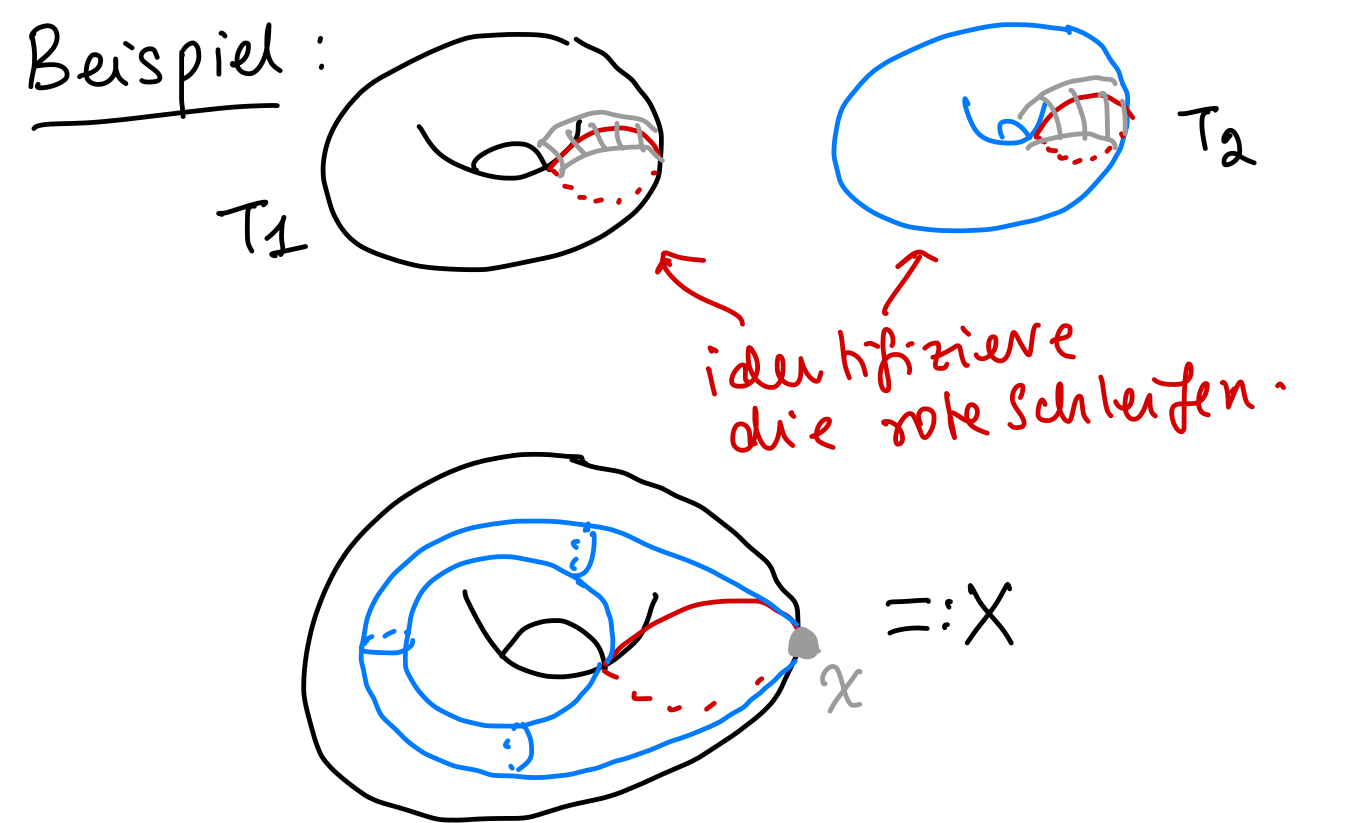
\includegraphics[scale=0.25]{figures/handdrawn/torus-mit-torus-verklebt.png}
    \end{minipage}
    
    Formal definieren wir $X$ durch
     \[
         X\coloneqq \faktor{S^1 \times  S^1 \times \left \{1\right\} \sqcup S^1 \times S^1 \times  \left \{2\right\} }{S^1 \times \left \{1\right\} \times \left \{1\right\} \sim  S^1 \times \left \{1\right\} \times \left \{2\right\} }
    .\] 
    Wir würden jetzt gerne $T_1,T_2$ (die Tori) in $X$ verwenden und \nameref{thm:seifert-van-kampen} anwenden, aber diese sind nicht offen. Wir müssen die Tori also 'etwas' vergrößern, sodass sie offen sind, ohne dass wir die schönen Eigenschaften der Tori verlieren. Man gelangt zu:
    \begin{IEEEeqnarray*}{rCl}
        A_1 &\coloneqq&  S^1 \times (e^{-i\theta}, e^{i\theta}) \subset T_1 \\
        A_2        & \coloneqq  & S^1 \times  (e^{-i\theta}, e^{i\theta}) \subset T_2 \\
        U_1 & \coloneqq  & T_1 \cup A_2  \simeq T_1\\
        U_2 &\coloneqq & T_2 \cup A_1 \simeq T_2
    \end{IEEEeqnarray*}
    Die Homotopieäquivalenz erhalten wir einfach durch stetiges zusammenziehen dieses 'angeklebten' Schlauches $A_i$.

    Jetzt sind also  $U_1,U_2$ offen und verhalten sich wie unsere Tori, und der Schnitt ergibt sich als $U_3 \coloneqq  U_1 \cap  U_2 = A_1 \cup A_2$, und dieser ist auch wegzusammenhängend.

    Also ergibt sich nun mit \nameref{thm:seifert-van-kampen}, dass
    \[
        \pi_1(X) \cong \pi_1(U_1,x ) \star_{\pi_1(U_3,x)} \pi_1(U_2, x) 
    .\] 

Da wir schon wissen, dass $\pi_1(T_1) \cong \mathbb{Z} \times  \mathbb{Z}$ die Fundamentalgruppe des Torus ist, und das lässt sich darstellen als
\begin{IEEEeqnarray*}{rCl}
    \pi_1(T_1) & = & \left< a,b \mid  ab a^{-1} b^{-1} \right> \\
    \pi_1(T_2)               & = & \left< c,d \mid  cdc^{-1}d^{-1} \right> 
\end{IEEEeqnarray*}
Man überlegt sich noch, dass $U_3 = A_1 \cup A_2 \simeq S^1$, auch indem wir die extra 'Schläuche' stetig verkürzen, also $\pi_1(U_3) = \mathbb{Z} = \left< γ \mid  \right> $.
\begin{IEEEeqnarray*}{rCl}
    \pi_1(X,x) & = & \left< a,b,c,d \mid  aba^{-1}b^{-1}, cdc^{-1}d^{-1}, a  =  c \right> \\
                                                                            & = & \left< a,b,c,d \mid aba^{-1}b^{-1}, cdc^{-1}d^{-1}, ac^{-1} \right> 
\end{IEEEeqnarray*}
\begin{oral}
    Man kann auch eine andere Darstellung von $X$ wählen, indem wir die 'lange' Schleife von  $X$ wählen (die in Wahrheit aber natürlich Symmetrisch ist). Dann kann man sich  $X$ als 'Stapel von Donuts' vorstellen, die einfach übereinander liegen und sich kanonisch berühren. Dann sieht man auch, dass
     \[
         X = (S^1 \twedge S^1 ) \times S^1
    .\] 
    und wir würden schnell erhalten, dass
    \begin{IEEEeqnarray*}{rCl}
        \pi_1(X) & = & \pi_1(S^1 \twedge S^1) \times  \pi(S^1) \\
                 & = & \left< b,d\mid  \right> \times \left< a\mid  \right> \\
                 & = & \left< a,b,d\mid aba^{-1}b^{-1}, ada^{-1}d^{-1} \right> 
    \end{IEEEeqnarray*}
    Man sieht auch leicht, dass die beiden Darstellungen, die wir erhalten haben, die gleichen Gruppen beschreiben.
\end{oral}
\end{example}

\begin{dnotation}[Freie Gruppen]
    Die Notation $\left< a \mid  \right> $ heißt natürlich, dass wir keine Relationen fordern, also $\left<  a \mid  \right>  \cong \mathbb{Z}$. Manchmal lässt man diesen Strich dann auch weg, und schreibt einfach sofort
    \[
    \left< a \right>  \cong \mathbb{Z}
    .\] 
    Das darf man aber nicht verwechseln mit der von $g$ erzeugten Untergruppe, wenn  $g\in G$ bereits ein Element ist, hier erhalten wir natürlich implizit alle Relationen, die $g$ als Element von $G$ besitzt.
\end{dnotation}

\begin{remark*}
    Vorlesung 21 setzt hier direkt mit CW-Komplexen, d.h. \autoref{sec:cw-komplexe} fort. Wir geben hier direkt den Rest von \autoref{sec:seifert-van-kampen} wieder.
\end{remark*}
